%If you have a single appendix, you need to change {\chapter*{APPENDIX: THIS IS THE FIRST APPENDIX}
%to {\chapter*{APPENDIX: YOUR APPENDIX TITLE HERE} if you have two or more appendices
%you need to change {\chapter{THIS IS THE FIRST APPENDIX}} to
%{\chapter{YOUR APPENDIX TITLE HERE}}
%
%If you make these changes correctly Latex will complain bitterly about the additions to the TOC
%but will make them correctly in a manner acceptable to the Editorial Office.

\ifthenelse{\value{noa} = 1}
%...................then
{\chapter*{APPENDIX: STRUCTURED OVERLAY BROADCAST}
\label{broadcast}
\addcontentsline{toc}{chapter}{APPENDIX: STRUCTURED OVERLAY BROADCAST}
\chaptermark{Appendix}
\markboth{Appendix}{Appendix}
\setcounter{chapter}{1}}
%...................else
{\chapter{STRUCTURED OVERLAY BROADCAST}
\label{broadcast}}
%...................

\begin{figure}[ht]
\centering
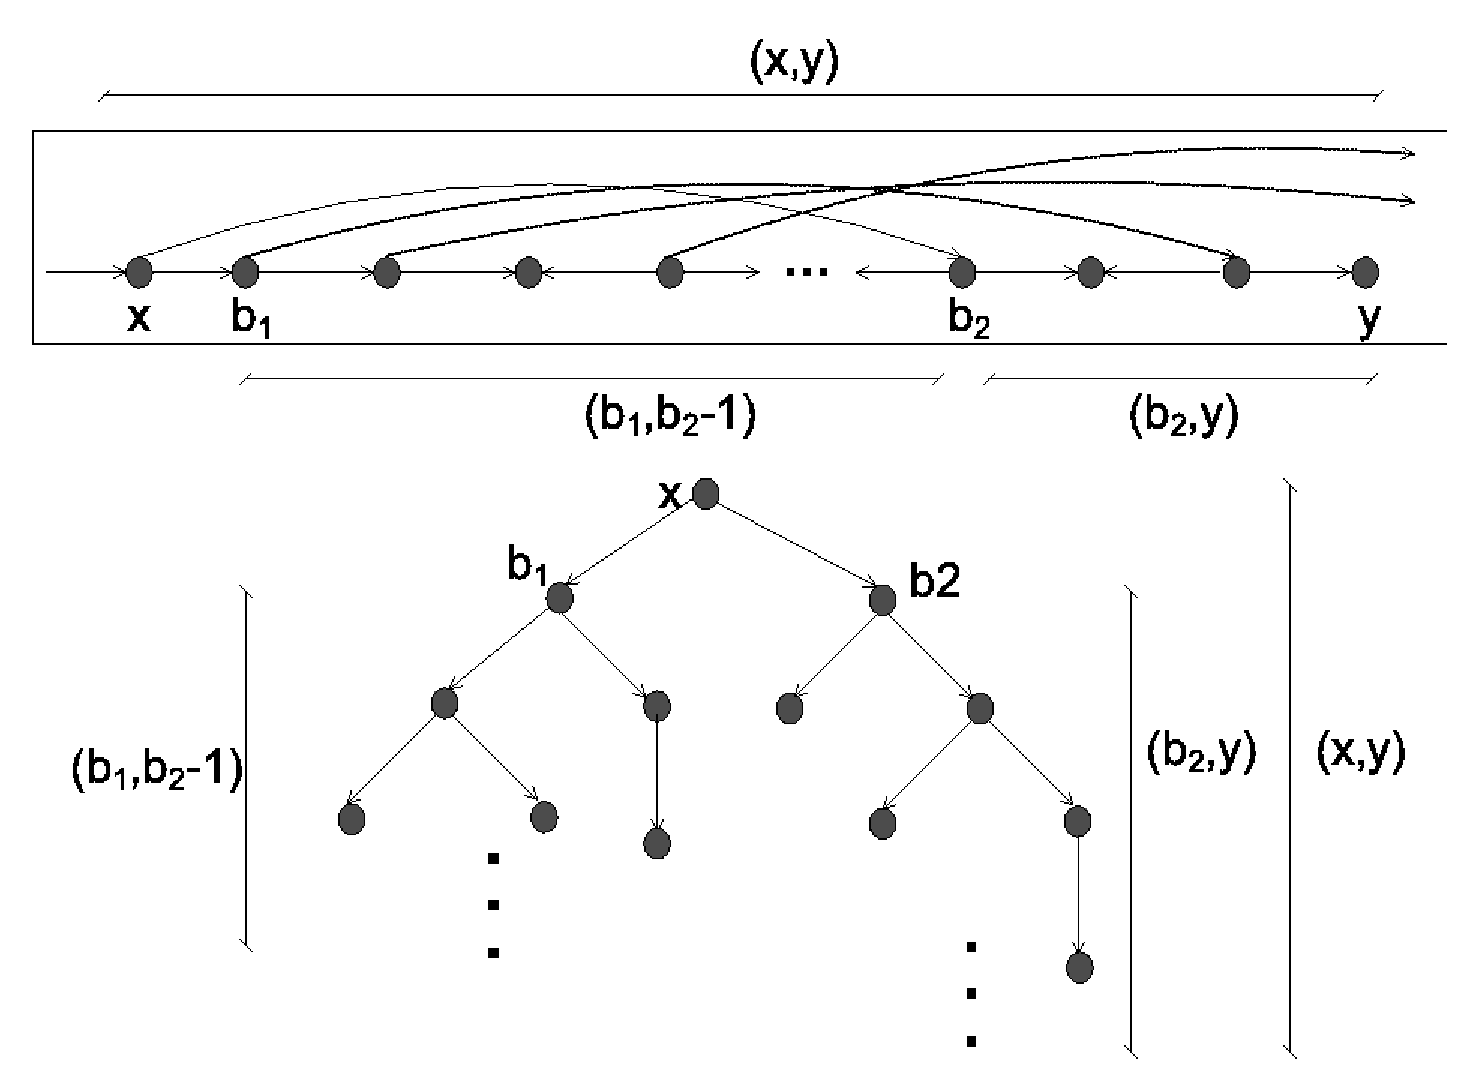
\includegraphics[width=4in]{figs/tree.eps}
\caption[Tree-based overlay broadcast]{Tree-based overlay broadcast}
\label{fig:tree}
\end{figure}  

Broadcast revocation can be used to address the deficiencies of DHT revocation.
As a topic of previous research works~\cite{broadcast, chord_broadcast},
structured overlays can be used without additional state to perform efficient
broadcasts from any point in the overlay to the entire overlay.  In these
papers, analysis and simulations have shown that the approach can be completed
in a network size of $n$ in $O(\log^2 n)$ time with $n$ messages.  The overlay
broadcast algorithm used in this paper provides a complete overlay broadcast in
$O(\log^2 n)$ time with $n$ messages.  When applied to Brunet, as illustrated
in Figure~\ref{fig:tree}, it utilizes the organization of a structured system
with a circular address space that requires peers be connected to those whose
node addresses are the closest to their own, features typical of
one-dimensional structured overlays including Chord~\cite{chord},
Pastry~\cite{pastry}, and Symphony.  Using such an organization, it is possible
to do perform a broadcast with no additional state.  To perform a broadcast,
each node performs the following recursive algorithm:

\begin{algorithmic}
\STATE {\bf BROADCAST(start, end, message)}:
  \STATE RECEIVE(message)
  \FOR{$i$ in length(connections)}
    \STATE n\_start $\gets$ ADDRESS(connections$[i]$)
    \IF {n\_start $\not\in$ $[$start, end$)$}
      \STATE continue
    \ENDIF
    \STATE n\_end $\gets$ ADDRESS(connections$[i+1]$)
    \IF {n\_end $\not\in$ $[$start, end$)$}
      \STATE n\_end $\gets$ end
    \ENDIF
    \STATE msg $\gets$ (BROADCAST, n\_start, n\_end, message)
    \STATE SEND(connections$[i]$, msg)
  \ENDFOR
\end{algorithmic}
with ``connections'' as a circular list of connections in non-decreasing order
from the perspective of the node performing the current recursive, broadcast
step.

In this algorithm, the broadcast initiator uses its own address as the start
and end, thus the broadcast will span the entire overlay after completing
recursive calls at each connected node.  A recursive end, ``n\_end'', must be
inside the region between ``start'' and ``end'', thus if the connection
following the current sending connection, ``connections$[i+1]$'', is not in
that region, it will only broadcast up to ``end'' and not the address specified
by that connection.  To summarize, the overlay is recursively partitioned
amongst the nodes at each hop in the broadcast.  By doing so, all nodes receive
the broadcast without receiving duplicate broadcast messages.
